\documentclass{ctexart}
\usepackage[utf8]{inputenc}
\usepackage{graphicx}
\usepackage{amsmath}
\usepackage{amssymb}
\usepackage{enumitem}
\usepackage{xcolor}
\usepackage{listings}
\newfontfamily\courier{Courier New}
\lstset{linewidth=1.1\textwidth,
        numbers=left, %设置行号位置 
        basicstyle=\small\courier,
        numberstyle=\tiny\courier, %设置行号大小  
        keywordstyle=\color{blue}\courier, %设置关键字颜色  
        %identifierstyle=\bf,
        commentstyle=\it\color[cmyk]{1,0,1,0}\courier, %设置注释颜色 
        stringstyle=\it\color[RGB]{128,0,0}\courier,
        %framexleftmargin=10mm,
        frame=single, %设置边框格式  
        backgroundcolor=\color[RGB]{245,245,244},
        %escapeinside=``, %逃逸字符(1左面的键),用于显示中文  
        breaklines, %自动折行  
        extendedchars=false, %解决代码跨页时,章节标题,页眉等汉字不显示的问题  
        xleftmargin=2em,xrightmargin=2em, aboveskip=1em, %设置边距  
        tabsize=4, %设置tab空格数  
        showspaces=false %不显示空格  
        basicstyle=\small\courier
       }  

\title{数值分析 - 第三章实验报告}
\author{强基数学2001班 樊睿}
\date{December 19,2022}

\begin{document}

\maketitle

\section{abstract}

本项目分别用 ppform 和 B-spline 实现了分段线性样条和三次样条的函数拟合和曲线拟合。

\section{ppform的理论及实现}

ppform 使用传统的待定系数方法,对除右端点外的结点 $x_0,x_1,\dots,x_{n-1}$(注:本文结点标号全部从 $0$ 到 $n$,即结点总数为 $n+1$)求出样条在结点处的 $0$ 至 $m$ 次导数值,然后利用泰勒展开式求出每段的函数解析式。

本节完整程序见 \verb|Spline.h|。

\subsection{分段线性样条 $\mathbb{S}_1^0$}

\subsubsection{问题描述}

已知结点处 $a=x_0<x_1<\dots<x_{n-1}<x_n=b$ 的函数值 $f(x_0)=y_0,f(x_1)=y_1,\dots,f(x_n)=y_n$,用分段线性样条 $s(x)\in \mathbb{S}_1^0$ 拟合 $f$。

\subsubsection{理论基础}

设样条在结点 $(x_i,x_{i+1}$ 之间的解析式是 $s(x)=y_i+K_i(x_i)(x-x_i)$,则 $K_i=\dfrac{y_{i+1}-y_i}{x_{i+1}-x_i}$。

\subsubsection{代码实现}

设计 \verb|LinearSpline| 类。
\begin{itemize}
\item \verb|vector<type>| 型私有成员变量 \verb|x|:结点坐标。
\item \verb|vector<type>| 型私有成员变量 \verb|f|:结点函数值。
\item 构造函数 \verb|LinearSpline(const vector<type>& x, const vector <type>& f)|:默认构造。
\item \verb|type| 型公有成员函数 \verb|GetValue(const type& _x)|:获取样条函数在 \verb|_x| 处的拟合值。用STL自带的\verb|upper_bound|函数定位到代求点所在区间后直接取值即可。
\end{itemize}

具体代码实现如下。同时还支持了对具体函数 $f$ 在区间 $[l,r]$ 进行 $n+1$ 个结点的等距插值。
\begin{lstlisting}[language={c++}]
template <class type>
class LinearSpline {
private:
	vector <type> x, f;	// 结点,函数值
public:
	LinearSpline(const vector<type>& x, const vector<type>& f) : x(x), f(f) {}
	type GetValue(const type& _x) {
		int i = upper_bound(x.begin(), x.end(), _x) - x.begin() - 1;
		type t = _x - x[i], c0 = f[i], c1 = (f[i+1] - f[i]) / (x[i+1] - x[i]);
		return c0 + c1 * t;
	}
};

template <class type>
LinearSpline<type> LinearSplineInterpolation(const Function <type>& f, const type& l, const type& r, const int& n) {
	vector <type> x(n+1), y(n+1);
	for(int i = 0; i <= n; ++ i) x[i] = l + (r - l) / n * i, y[i] = f(x[i]);
	return LinearSpline<type>(x, y);
}
\end{lstlisting}

\subsection{分段三次样条}

\subsubsection{问题描述}

已知结点处 $a=x_0<x_1<\dots<x_{n-1}<x_n=b$ 的函数值 $f(x_0)=y_0,f(x_1)=y_1,\dots,f(x_n)=y_n$ 和端点处对一阶或二阶导数的限制(自然样条、完全样条、端点处二阶导指定的样条),用分段线性样条 $s(x)\in \mathbb{S}_3^2$ 拟合 $f$。

\subsubsection{理论基础}

设样条在结点 $(x_i,x_{i+1})$ 之间的解析式是 $s(x)=y_i+m_i(x-x_i)+\dfrac{M_i}2(x-x_i)^2+\dfrac{M_{i+1}-M_i}{6(x_{i+1}-x_i)}(x-x_1)^3$。

当求自然样条或完全样条,即 $m_0=f[x_0,x_0]$ 和 $m_n=f[x_n,x_n]$ 给定时,由讲义的 Lem 3.4,Lem 3.6 可得 $M_i$ 满足如下关系式:

\begin{equation}
\begin{bmatrix}
2 & 1 & & & & \\
\lambda_1 & 2 & \mu_1 & & & \\
& \lambda_2 & 2 & \mu_2 & \\
& \ddots & \ddots & \ddots & \\
& & & \lambda_{n-1} & 2 & \mu_{n-1} \\
& & & & 1 & 2\\
\end{bmatrix}
\begin{bmatrix}
M_0\\
M_1\\
M_2\\
\vdots\\
M_{n-1}\\
M_n\\
\end{bmatrix}
=
6\begin{bmatrix}
f[x_0,x_0,x_1]\\
f[x_0,x_1,x_2]\\
f[x_1,x_2,x_3]\\
\vdots\\
f[x_{n-2},x_{n-1},x_n]\\
f[x_{n-1},x_n,x_n]\\
\end{bmatrix}
\end{equation}

其中,$\lambda_i=\dfrac{x_i-x_{i-1}}{x_{i+1}-x_{i-1}}$,$\mu_i=\dfrac{x_{i+1}-x_i}{x_{i+1}-x_{i-1}}$,右边所有的二阶差商都可以直接计算。

然后根据 Lem 3.4 求 $m_i$:

\begin{equation}
\begin{aligned}
    & m_i=f[x_i,x_{i+1}]-\dfrac 16 (M_{i+1}+2M_i)(x_{i+1}-x_i), & i=0,1,\dots,n-1\\
    & m_n=f[x_n,x_{n-1}]-\dfrac 16 (M_{n-1}+2M_n)(x_{n-1}-x_n), & i=n
\end{aligned}
\end{equation}

当求端点处二阶导给定的样条,即 $M_0$ 和 $M_n$ 给定时,$f[x_0,x_0,x_1]$ 和 $f[x_{n-1},x_{n-1},x_n]$ 未知但不再需要,只需去掉第一个和最后一个方程,解一个 $n-1$ 阶线性方程组即可。

\subsubsection{代码实现}

设计 \verb|CubicSpline| 类。

\begin{itemize}
\item \verb|vector<type>| 型私有成员变量 \verb|x,f,m,M|:结点坐标、函数值、一阶导、二阶导。
\item 构造函数 \verb|CubicSpline(const vector<type>& x, const vector <type>& f, const string& mode, const type& m0, const type& mn)|:构造函数。mode 可选择 \verb|Natural|、\verb|Complete| 或 \verb|Specified_Second_Derivatives|,\verb|m0| 和 \verb|mn| 是端点处的一阶或二阶导数值。具体实现时先计算二阶差商,然后解三对角方程组求出 $M_i$,最后求 $m_i$。
\item \verb|type| 型公有成员函数 \verb|GetValue(const type& _x)|:获取样条函数在 \verb|_x| 处的拟合值。用STL自带的\verb|upper_bound|函数定位到代求点所在区间后直接取值即可。
\end{itemize}

具体代码实现如下。同时还支持了对具体函数 $f$ 在区间 $[l,r]$ 进行 $n+1$ 个结点的等距插值。

\begin{lstlisting}[language={c++}]
template <class type>
class CubicSpline {
private:
	vector <type> x, f, m, M;	// 结点, 函数值, 一阶导, 二阶导
public:
	CubicSpline(const vector<type>& x, const vector<type>& f, const string& mode = "Natural", const type& m0 = 0, const type& mn = 0) : x(x), f(f) {
		int n = x.size() - 1;
		m.resize(n+1);
		vector <type> l(n+1), u(n+1);	// lambda, mu
		for (int i = 1; i <= n-1; ++ i) {
			l[i] = (x[i] - x[i-1]) / (x[i+1] - x[i-1]);
			u[i] = (x[i+1] - x[i]) / (x[i+1] - x[i-1]);
		}

		vector <type> dq1(n+1), dq2(n+2);	// 一阶差商, 二阶差商
		vector <type> a(n+1), b(n), c(n), y(n+1);

		if (mode == "Natural" && (m0 != 0 || mn != 0)) throw "Invalid Parameter!";
		if (mode == "Complete" || mode == "Natural") {
			// 计算差商
			for (int i = 1; i <= n; ++ i)
				dq1[i] = (f[i] - f[i-1]) / (x[i] - x[i-1]);
			dq2[1] = (dq1[1] - m0) / (x[1] - x[0]);
			for (int i = 2; i <= n; ++ i)
				dq2[i] = (dq1[i] - dq1[i-1]) / (x[i] - x[i-2]);
			dq2[n+1] = (mn - dq1[n]) / (x[n] - x[n-1]);
			// 构造三对角方程组
			for (int i = 1; i <= n-1; ++ i) {
				a[i] = 2;
				b[i-1] = u[i];
				c[i] = l[i];
				y[i] = 6 * dq2[i+1];
			}
			a[0] = 2, c[0] = 1, y[0] = 6 * dq2[1];
			a[n] = 2, b[n-1] = 1, y[n] = 6 * dq2[n+1];
			// 调用 Thomas 算法解出结点处的二阶导 M
			M = Thomas(a, b, c, y);
			// 根据 M 的值计算 m
			m[0] = m0, m[n] = mn;
			for (int i = 1; i <= n-1; ++ i)
				m[i] = dq1[i+1] - (2 * M[i] + M[i+1]) * (x[i+1] - x[i]) / 6;
		}
		else if (mode == "Specified_Second_Derivatives") {
			// 计算差商
			for (int i = 1; i <= n; ++ i)
				dq1[i] = (f[i] - f[i-1]) / (x[i] - x[i-1]);
			for (int i = 2; i <= n; ++ i)
				dq2[i] = (dq1[i] - dq1[i-1]) / (x[i] - x[i-2]);
			// 构造三对角方程组
			for (int i = 1; i <= n-1; ++ i) {
				a[i] = 2;
				b[i-1] = u[i];
				c[i] = l[i];
				y[i] = 6 * dq2[i+1];
			}
			a[0] = 1, y[0] = m0;
			a[n] = 1, y[n] = mn;
			// 调用 Thomas 算法解出结点处的二阶导 M
			M = Thomas(a, b, c, y);
			// 根据 M 的值计算 m
			for (int i = 0; i <= n-1; ++ i)
				m[i] = dq1[i+1] - (2 * M[i] + M[i+1]) * (x[i+1] - x[i]) / 6;
			m[n] = dq1[n] - (2 * M[n] + M[n-1]) * (x[n-1] - x[n]) / 6;
		}
	}
	type GetValue(const type& _x) const {
		// 求出 x 所在结点区间,根据该区间上的解析式计算样条函数的值
		int i = upper_bound(x.begin(), x.end(), _x) - x.begin() - 1;
		type t = _x - x[i], c0 = f[i], c1 = m[i], c2 = M[i] / 2, c3 = (M[i+1] - M[i]) / (x[i+1] - x[i]) / 6;
		return c0 + t * (c1 + t * (c2 + c3 * t));
	}
};

template <class type>
CubicSpline<type> CubicSplineInterpolation(const Function <type>& f, const type& l, const type& r, const int& n, const string& mode = "Natural") {
	vector <type> x(n+1), y(n+1);
	for(int i = 0; i <= n; ++ i) x[i] = l + (r - l) / n * i, y[i] = f(x[i]);
	type m0, mn;
	if (mode == "Natural") m0 = mn = 0;
	else if (mode == "Complete") m0 = f.d(l), mn = f.d(r);
	else if (mode == "Specified_Second_Derivatives") m0 = f.d(l, 2), mn = f.d(r, 2);
	return CubicSpline<type>(x, y, mode, m0, mn);
}
\end{lstlisting}

另外附上解三对角方程组的程序(见 \verb|Thomas.h|):

\begin{lstlisting}[language={c++}]
#include <bits/stdc++.h>
using namespace std;

template <class type>
vector<type> Thomas(vector<type>& a, vector<type>& b, vector<type>& c, vector<type> y) {
	int n = a.size();
	if (b.size() != n-1 || c.size() != n-1) throw "Invalid Size!";
	vector<type> p(n), q(n-1);
	p[0] = a[0];
	for (int i = 1; i < n; ++ i) {
		q[i-1] = c[i-1] / p[i-1];
		p[i] = a[i] - b[i-1] * q[i-1];
	}
	y[0] = y[0] / p[0];
	for (int i = 1; i < n; ++ i)
		y[i] = (y[i] - b[i-1] * y[i-1]) / p[i];
	for (int i = n-2; i >= 0 ; -- i)
		y[i] = y[i] - q[i] * y[i+1];
	return y;
}
\end{lstlisting}

\subsection{实例测试(A题)}

对于题中函数,简单计算可得其一二阶导数如下:

\begin{gather}
f'(x)=\dfrac {-50x}{(1+25x^2)^2} \\
f''(x)=\dfrac {-50+1250x^2}{(1+25x^2)^3}
\end{gather}

然后直接调用对应函数,将插值结果输出到 \verb|csv| 中,再用 python 读取并输出,测试线性样条和三次样条的拟合效果。

\begin{lstlisting}[language={c++}]
#include <bits/stdc++.h>
#include "Spline.h"
#include "../HW1/function.h"
using namespace std;

class F : public Function<double> {
	virtual double operator () (const double& x) const {
		return 1 / (1 + 25*x*x);
	}
	virtual double d (const double& x, const int& k = 1) const {
		if (k == 1) return -50 * x / (1 + 25*x*x) / (1 + 25*x*x);
		else if (k == 2) return (-50 + 1250*x*x) / (1 + 25*x*x) / (1 + 25*x*x) / (1 + 25*x*x);
		else throw 0;
	}
} f;

int main() {
	LinearSpline<double> A1 = LinearSplineInterpolation<double>(f, -1.0, 1.0, 5);
	LinearSpline<double> A2 = LinearSplineInterpolation<double>(f, -1.0, 1.0, 10);
	LinearSpline<double> A3 = LinearSplineInterpolation<double>(f, -1.0, 1.0, 20);
	LinearSpline<double> A4 = LinearSplineInterpolation<double>(f, -1.0, 1.0, 40);
	LinearSpline<double> A5 = LinearSplineInterpolation<double>(f, -1.0, 1.0, 80);

	ofstream out1("a1.csv");
	out1 << "x,y" << '\n';
	for(int i = -999; i <= 999; ++ i) out1 << i * 0.001 << ',' << A1.GetValue(i * 0.001) << '\n';
	ofstream out2("a2.csv");
	out2 << "x,y" << '\n';
	for(int i = -999; i <= 999; ++ i) out2 << i * 0.001 << ',' << A2.GetValue(i * 0.001) << '\n';
	ofstream out3("a3.csv");
	out3 << "x,y" << '\n';
	for(int i = -999; i <= 999; ++ i) out3 << i * 0.001 << ',' << A3.GetValue(i * 0.001) << '\n';
	ofstream out4("a4.csv");
	out4 << "x,y" << '\n';
	for(int i = -999; i <= 999; ++ i) out4 << i * 0.001 << ',' << A4.GetValue(i * 0.001) << '\n';
	ofstream out5("a5.csv");
	out5 << "x,y" << '\n';
	for(int i = -999; i <= 999; ++ i) out5 << i * 0.001 << ',' << A5.GetValue(i * 0.001) << '\n';

	CubicSpline<double> A6 = CubicSplineInterpolation<double>(f, -1.0, 1.0, 5, "Complete");
	CubicSpline<double> A7 = CubicSplineInterpolation<double>(f, -1.0, 1.0, 10, "Complete");
	CubicSpline<double> A8 = CubicSplineInterpolation<double>(f, -1.0, 1.0, 20, "Complete");
	CubicSpline<double> A9 = CubicSplineInterpolation<double>(f, -1.0, 1.0, 40, "Complete");
	CubicSpline<double> A10 = CubicSplineInterpolation<double>(f, -1.0, 1.0, 80, "Complete");
	
	ofstream out6("a6.csv");
	out6 << "x,y" << '\n';
	for(int i = -999; i <= 999; ++ i) out6 << i * 0.001 << ',' << A6.GetValue(i * 0.001) << '\n';
	ofstream out7("a7.csv");
	out7 << "x,y" << '\n';
	for(int i = -999; i <= 999; ++ i) out7 << i * 0.001 << ',' << A7.GetValue(i * 0.001) << '\n';
	ofstream out8("a8.csv");
	out8 << "x,y" << '\n';
	for(int i = -999; i <= 999; ++ i) out8 << i * 0.001 << ',' << A8.GetValue(i * 0.001) << '\n';
	ofstream out9("a9.csv");
	out9 << "x,y" << '\n';
	for(int i = -999; i <= 999; ++ i) out9 << i * 0.001 << ',' << A9.GetValue(i * 0.001) << '\n';
	ofstream out10("a10.csv");
	out10 << "x,y" << '\n';
	for(int i = -999; i <= 999; ++ i) out10 << i * 0.001 << ',' << A10.GetValue(i * 0.001) << '\n';

	CubicSpline<double> A11 = CubicSplineInterpolation<double>(f, -1.0, 1.0, 5, "Natural");
	CubicSpline<double> A12 = CubicSplineInterpolation<double>(f, -1.0, 1.0, 10, "Natural");
	CubicSpline<double> A13 = CubicSplineInterpolation<double>(f, -1.0, 1.0, 20, "Natural");
	CubicSpline<double> A14 = CubicSplineInterpolation<double>(f, -1.0, 1.0, 40, "Natural");
	CubicSpline<double> A15 = CubicSplineInterpolation<double>(f, -1.0, 1.0, 80, "Natural");
	
	ofstream out11("a11.csv");
	out11 << "x,y" << '\n';
	for(int i = -999; i <= 999; ++ i) out11 << i * 0.001 << ',' << A11.GetValue(i * 0.001) << '\n';
	ofstream out12("a12.csv");
	out12 << "x,y" << '\n';
	for(int i = -999; i <= 999; ++ i) out12 << i * 0.001 << ',' << A12.GetValue(i * 0.001) << '\n';
	ofstream out13("a13.csv");
	out13 << "x,y" << '\n';
	for(int i = -999; i <= 999; ++ i) out13 << i * 0.001 << ',' << A13.GetValue(i * 0.001) << '\n';
	ofstream out14("a14.csv");
	out14 << "x,y" << '\n';
	for(int i = -999; i <= 999; ++ i) out14 << i * 0.001 << ',' << A14.GetValue(i * 0.001) << '\n';
	ofstream out15("a15.csv");
	out15 << "x,y" << '\n';
	for(int i = -999; i <= 999; ++ i) out15 << i * 0.001 << ',' << A15.GetValue(i * 0.001) << '\n';

	CubicSpline<double> A16 = CubicSplineInterpolation<double>(f, -1.0, 1.0, 5, "Specified_Second_Derivatives");
	CubicSpline<double> A17 = CubicSplineInterpolation<double>(f, -1.0, 1.0, 10, "Specified_Second_Derivatives");
	CubicSpline<double> A18 = CubicSplineInterpolation<double>(f, -1.0, 1.0, 20, "Specified_Second_Derivatives");
	CubicSpline<double> A19 = CubicSplineInterpolation<double>(f, -1.0, 1.0, 40, "Specified_Second_Derivatives");
	CubicSpline<double> A20 = CubicSplineInterpolation<double>(f, -1.0, 1.0, 80, "Specified_Second_Derivatives");

	ofstream out16("a16.csv");
	out16 << "x,y" << '\n';
	for(int i = -999; i <= 999; ++ i) out16 << i * 0.001 << ',' << A16.GetValue(i * 0.001) << '\n';
	ofstream out17("a17.csv");
	out17 << "x,y" << '\n';
	for(int i = -999; i <= 999; ++ i) out17 << i * 0.001 << ',' << A17.GetValue(i * 0.001) << '\n';
	ofstream out18("a18.csv");
	out18 << "x,y" << '\n';
	for(int i = -999; i <= 999; ++ i) out18 << i * 0.001 << ',' << A18.GetValue(i * 0.001) << '\n';
	ofstream out19("a19.csv");
	out19 << "x,y" << '\n';
	for(int i = -999; i <= 999; ++ i) out19 << i * 0.001 << ',' << A19.GetValue(i * 0.001) << '\n';
	ofstream out20("a20.csv");
	out20 << "x,y" << '\n';
	for(int i = -999; i <= 999; ++ i) out20 << i * 0.001 << ',' << A20.GetValue(i * 0.001) << '\n';

}
\end{lstlisting}

作图程序略,详见 \verb|plot.ipynb|。

分段线性样条、自然三次样条、完全三次样条、端点处二阶导指定的三次样条的拟合效果见图\ref{fig1}、\ref{fig2}、\ref{fig3}、\ref{fig4}。蓝色虚线为 $f(x)$,黄色、绿色、红色、紫色和棕色分别为 $n=5,10,20,40,80$ 的样条曲线。

\begin{figure}[htbp]
\centering
\begin{minipage}{5cm}
    \centering
    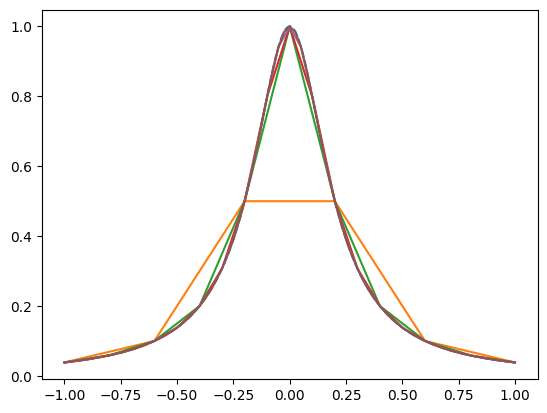
\includegraphics[width=5cm]{a1.png}
    \caption{线性}
    \label{fig1}
\end{minipage}
\qquad
\begin{minipage}{5cm}
    \centering
    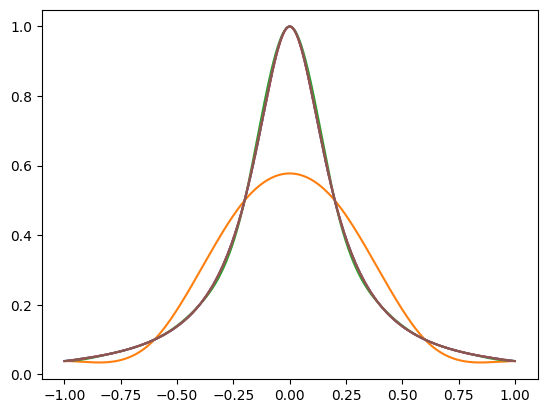
\includegraphics[width=5cm]{a3.png}
    \caption{自然}
    \label{fig2}
\end{minipage}
\begin{minipage}{5cm}
    \centering
    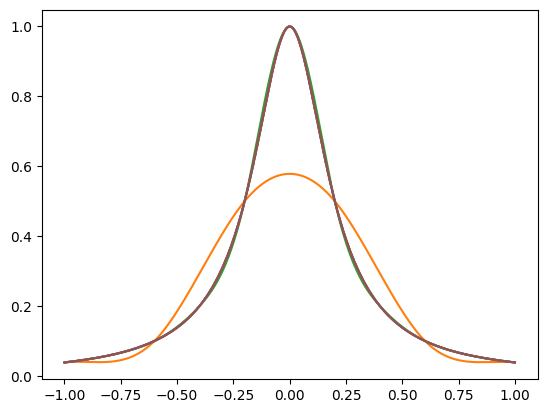
\includegraphics[width=5cm]{a2.png}
    \caption{完全}
    \label{fig3}
\end{minipage}
\qquad
\begin{minipage}{5cm}
    \centering
    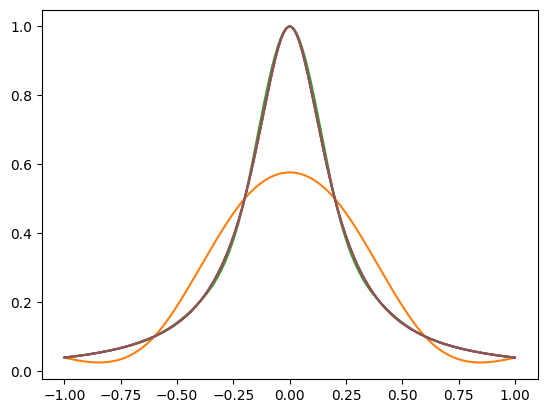
\includegraphics[width=5cm]{a4.png}
    \caption{端点处二阶导指定}
    \label{fig4}
\end{minipage}
\end{figure}

分段样条的拟合偏差较大,但在 $n\geq 20$ 时基本无误差。其他三者的拟合在 $n\geq 10$ 及以上时基本无误差。

\section{B-Spline的理论及实现(B题)}

B-Spline 通过将样条函数分解成 $n+m$ 个 $m$ 阶B-样条基函数的线性组合,可以解决结点为整数的插值问题。进而通过简单的平移和放缩变换也可以解决任意结点间隔相等的插值问题。多数情形下,我们只需要用到一阶、二阶和三阶B-Spline。本项目仅支持结点为整数的B-Spline插值。

\subsection{B-Spline的基函数}

经典B-Spline的基函数可通过递归定义。

\begin{equation}
    B_{i,\mathbb{Z}}^{n+1}(x)=\dfrac{x-i+1}{n+1}B_{i,\mathbb{Z}}^n(x)+\dfrac{i+n+1-x}{n+1}B_{i+1,\mathbb{Z}}^n(x)
\end{equation}

当 $m=1,2,3$ 时,也可以直接写出它们的表达式。

\begin{equation}
B_{i,\mathbb{Z}}^1(x)=\left\{
\begin{aligned}
    & x-i+1, & i-1\leq x\leq i\\
    & i+1-x, & i\leq x\leq i+1\\
    & 0, & \text{others}\\
\end{aligned}
\right.
\end{equation}

\begin{equation}
B_{i,\mathbb{Z}}^2(x)=\left\{
\begin{aligned}
    & \dfrac{(x-i+1)^2}2, & i-1\leq x\leq i\\
    & \dfrac 34 - (x-(i+\dfrac 12))^2, & i\leq x\leq i+1\\
    & \dfrac{(i+2-x)^2}2, & i+1\leq x\leq i+2\\
    & 0,\text{others}\\
\end{aligned}
\right.
\end{equation}

\begin{equation}
B_{i,\mathbb{Z}}^3(x)=\left\{
\begin{aligned}
    & \dfrac{(x-i+1)^3}6, & i-1\leq x\leq i\\
    & \dfrac 23 - \dfrac 12 (x-i+1)(i+1-x)^2, & i\leq x\leq i+1\\
    & B_{i,\mathbb{Z}}^3(2i+2-x), & i+1\leq x\leq i+3\\
    & 0, & \text{others}\\
\end{aligned}
\right.
\end{equation}

代码实现如下:

\begin{lstlisting}[language={c++}]
template <class type>
type B(const int& n, const int& i, const type& x) {
	if (n == 0) {
		if (i-1 < x && x <= i) return 1;
		else return 0;
	}
	// 根据 B 样条基的递归定义计算
	return (x-i+1) * B(n-1, i, x) / n + (i+n-x) * B(n-1, i+1, x) / n;
}
\end{lstlisting}

\subsection{用B-Spline实现分段线性样条}

\subsubsection{问题和理论基础}
条件和 ppform 相同,但要求结点为连续整数 $l,l+1,\dots,l+n$。

因为 $B_i^1(i)=1,B_i^1(j)=0,i\neq j$,所以
\begin{equation}
s(x)=\sum_{i=l}^{l+n}y_iB_i^1(i).
\end{equation}

\subsubsection{代码实现}

设计 \verb|LinearBSpline| 类。

\begin{itemize}
\item \verb|int| 型私有成员变量 \verb|L,R|:左右端点。
\item \verb|vector<type>| 型私有成员变量 \verb|coef|:基函数的系数。
\item 构造函数 \verb|LinearBSpline(const int& x0, const int& n, const vector<type>& f)|:\verb|L=x0,R=x0+n,coef=f|。
\item \verb|type| 型公有成员函数 \verb|GetValue(const type& _x)|:获取样条函数在 \verb|_x| 处的拟合值。用STL自带的\verb|upper_bound|函数定位到代求点所在区间后,取左右两个基函数值求和即可。
\end{itemize}

\begin{lstlisting}[language={c++}]
template <class type>
class LinearBSpline{
private:
	int L, R;
	vector<type> coef;
public:
	LinearBSpline(const int& x0, const int& n, const vector<type>& f) : L(x0), coef(f) {
		R = L + n;
	}
	type GetValue(const type& _x) const{
		if (_x < L || _x > R) throw "Out of Range!";
		int i = floor(_x);
		type res = 0;
		if(i   >= L && i   <= R) res += coef[i  -L] * B(1, i,   _x);
		if(i+1 >= L && i+1 <= R) res += coef[i+1-L] * B(1, i+1, _x);
		return res;
	}
};

template <class type>
LinearBSpline<type> LinearBSplineInterpolation(const Function <type>& f, const int& l, const int& n) {
	vector <type> y(n+1);
	for(int i = 0; i <= n; ++ i) y[i] = f(l+i);
	return LinearBSpline<type>(l, n, y);
}
\end{lstlisting}

\subsection{用B-Spline实现分段三次样条}

\subsubsection{问题和理论基础}
条件和 ppform 相同,但要求结点为连续整数 $l,l+1,\dots,l+n$。

设样条为 $s(x)=\sum_{i=-2}^na_iB_{i,\mathbb{Z}}^3(x)$。

对于自然样条和完全样条,根据讲义 Thm 3.57 可知,B-Spline 的系数满足方程组

\begin{equation}
\begin{aligned}
\begin{bmatrix}
2 & 1 & & & & \\
1 & 4 & 1 & & & \\
& 1 & 4 & 1 & \\
& \ddots & \ddots & \ddots & \\
& & & 1 & 4 & 1 \\
& & & & 1 & 2\\
\end{bmatrix}
\begin{bmatrix}
a_{-1}\\
a_0\\
a_1\\
\vdots\\
a_{n-1}\\
\end{bmatrix}
&=&
\begin{bmatrix}
3f(l)+f'(l)\\
6f(l+1)\\
6f(l+2)\\
\vdots\\
6f(l+n-1)\\
3f(l+n)-f'(l+n)\\
\end{bmatrix},\\
a_{-2}&=&a_0-2f'(l),\\
a_n&=&a_{n-2}+2f'(l+n).
\end{aligned}
\end{equation}

对于端点处二阶导指定的样条,根据三阶B-Spline的解析式可得它在整点处的二阶导数值为

\begin{equation}
B_{i,\mathbb{Z}}^3(i)=1,B_{i,\mathbb{Z}}^3(i+1)=-2,B_{i,\mathbb{Z}}^3(i+2)=1.
\end{equation}

因此有

\begin{equation}
f''(l)=a_{-2}-2a_{-1}+a_0,f''(l+n)=a_{n-2}-2a_{n-1}+a_n.
\end{equation}

进而可得

\begin{equation}
6a_{-1}=6f(l)-f''(l),6a_{n-1}=6f(l+n)-f''(l+n).
\end{equation}

用这两个方程代替上面矩阵中的第一个和最后一个方程即可。进而可求出 $a_{-2}$ 和 $a_n$ 的值。

\subsubsection{代码实现}

设计类 \verb|CubicBSpline|,

\begin{itemize}
\item \verb|int| 型私有成员变量 \verb|L,R|:左右端点。
\item \verb|vector<type>| 型私有成员变量 \verb|coef|:基函数的系数。
\item 构造函数 \verb|CubicSpline(const int& x, const int& n, const vector <type>& f, const string& mode, const type& m0, const type& mn)|:构造函数。mode 可选择 \verb|Natural|、\verb|Complete| 或 \verb|Specified_Second_Derivatives|,\verb|m0| 和 \verb|mn| 是端点处的一阶或二阶导数值。具体实现时先解三对角方程组求得中间 $n+1$ 个系数,再根据边界方程求出边界两个系数。
\item \verb|type| 型公有成员函数 \verb|GetValue(const type& _x)|:获取样条函数在 \verb|_x| 处的拟合值。用STL自带的\verb|upper_bound|函数定位到代求点所在区间后,取左右四个基函数值求和即可。
\end{itemize}

具体代码如下。

\begin{lstlisting}[language={c++}]
template <class type>
class CubicBSpline{
private:
	int L, R;
	vector <type> coef;
public:
	CubicBSpline(const int& x0, const int& n, const vector<type>& f, const string& mode = "Natural", const type& m0 = 0, const type& mn = 0) : L(x0) {
		R = L + n;
		vector <type> a(n+1), b(n), c(n), y(n+1);
		// 构造三对角方程组的中间 n-1 行
		for (int i = 1; i < n; ++ i) {
			a[i] = 4;
			b[i-1] = 1;
			c[i] = 1;
			y[i] = 6 * f[i];
		}
		// 根据边界条件构造首尾两行
		if (mode == "Natural" || mode == "Complete") {
			a[0] = 2, c[0] = 1, y[0] = 3 * f[0] + m0;
			a[n] = 2, b[n-1] = 1, y[n] = 3 * f[n] - mn;
			// 解出中间 n+1 个系数
			vector <type> t = Thomas(a, b, c, y);
			coef.resize(n+3);
			for (int i = 0; i <= n; ++ i) coef[i+1] = t[i];
			// 计算首尾两个系数
			coef[0] = coef[2] - 2 * m0;
			coef[n+2] = coef[n] + 2 * mn;
		}
		else if (mode == "Specified_Second_Derivatives") {
			a[0] = 6, y[0] = 6 * f[0] - m0;
			a[n] = 6, y[n] = 6 * f[n] - mn;
			// 解出中间 n+1 个系数
			vector <type> t = Thomas(a, b, c, y);
			coef.resize(n+3);
			for (int i = 0; i <= n; ++ i) coef[i+1] = t[i];
			// 计算首尾两个系数
			coef[0] = m0 - coef[2] + 2 * coef[1];
			coef[n+2] = mn - coef[n] + 2 * coef[n-1];
		}
	}
	type GetValue(const type& _x) const {
		if (_x < L || _x > R) throw "Out of Range!";
		int i = floor(_x);
		type res = 0;
		if(i-2 >= L-2 && i-2 <= R) res += coef[i-2-L+2] * B(3, i-2, _x);
		if(i-1 >= L-2 && i-1 <= R) res += coef[i-1-L+2] * B(3, i-1, _x);
		if(i   >= L-2 && i   <= R) res += coef[i  -L+2] * B(3, i  , _x);
		if(i+1 >= L-2 && i+1 <= R) res += coef[i+1-L+2] * B(3, i+1, _x);
		return res;
	}
};

template <class type>
CubicBSpline<type> CubicBSplineInterpolation(const Function <type>& f, const int& l, const int& n, const string& mode = "Natural") {
	vector <type> y(n+1);
	for(int i = 0; i <= n; ++ i) y[i] = f(l+i);
	type m0, mn;
	if (mode == "Natural") m0 = mn = 0;
	else if (mode == "Complete") m0 = f.d(l), mn = f.d(l+n);
	else if (mode == "Specified_Second_Derivatives") m0 = f.d(l, 2), mn = f.d(l+n, 2);
	return CubicBSpline<type>(l, n, y, mode, m0, mn);
}
\end{lstlisting}

\subsection{用B-Spline实现分段二次样条}

Thm 3.58 还提供了用分段二次样条在仅知道函数在端点和 $l+\dfrac 12,l+\dfrac 32,\dots,l+n-\dfrac 12$ 处的取值时的插值方法。这部分不是本项目的重点,因此仅给出类的设计代码。

设计 \verb|QuadraticBSpline| 类。

\begin{itemize}
\item \verb|int| 型私有成员变量 \verb|L,R|:左右端点。
\item \verb|vector<type>| 型私有成员变量 \verb|coef|:基函数的系数。
\item 构造函数 \verb|QuadraticBSpline(const int& x0, const int& n, const vector<type>& f, const type& f0, const type& fn)|:解三对角方程组求得基函数的中间 $n$ 个系数,再根据边界条件求出边界两个系数。
\item \verb|type| 型公有成员函数 \verb|GetValue(const type& _x)|:获取样条函数在 \verb|_x| 处的拟合值。用STL自带的\verb|upper_bound|函数定位到代求点所在区间后,取左右三个基函数值求和即可。
\end{itemize}

具体代码如下。

\begin{lstlisting}[language={c++}]
template <class type>
class QuadraticBSpline{
private:
	int L, R;
	vector <type> coef;
public:
	QuadraticBSpline(const int& x0, const int& n, const vector<type>& f, const type& f0, const type& fn) : L(x0) {
		R = L + n;
		vector <type> a(n), b(n-1), c(n-1), y(n);
		// 构造三对角方程组
		for (int i = 1; i < n-1; ++ i) {
			a[i] = 6;
			b[i-1] = 1;
			c[i] = 1;
			y[i] = 8 * f[i];
		}
		a[0] = 5, c[0] = 1, y[0] = 8 * f[0] - 2 * f0;
		a[n-1] = 5, b[n-2] = 1, y[n-1] = 8 * f[n-1] - 2 * fn;
		// 解出中间 n 个系数
		vector <type> t = Thomas(a, b, c, y);
		coef.resize(n+2);
		for (int i = 0; i < n; ++ i) coef[i+1] = t[i];
		// 计算首尾两个系数
		coef[0] = 2 * f0 - coef[1];
		coef[n+1] = 2 * fn - coef[n];
	}
	type GetValue(const type& _x) const {
		if (_x < L || _x > R) throw "Out of Range!";
		int i = floor(_x);
		type res = 0;
		if(i-1 >= L-1 && i-1 <= R) res += coef[i-1-L+1] * B(2, i-1, _x);
		if(i   >= L-1 && i   <= R) res += coef[i  -L+1] * B(2, i  , _x);
		if(i+1 >= L-1 && i+1 <= R) res += coef[i+1-L+1] * B(2, i+1, _x);
		return res;
	}
};

template <class type>
QuadraticBSpline<type> QuadraticBSplineInterpolation(const Function <type>& f, const int& l, const int& n) {
	vector <type> y(n);
	for(int i = 0; i < n; ++ i) y[i] = f(l+i+0.5);
	type f0 = f(l), fn = f(l+n);
	return QuadraticBSpline<type>(l, n, y, f0, fn);
}
\end{lstlisting}

\subsection{实例测试(C、D题)}

对于题中函数,简单计算可得其一二阶导数如下:

\begin{gather}
f'(x)=\dfrac {-2x}{(1+x^2)^2} \\
f''(x)=\dfrac {-2+6x^2}{(1+x^2)^3}
\end{gather}

然后直接调用对应函数,将插值结果输出到 \verb|csv| 中,再用 python 读取并输出,测试线性样条、三次样条和二次样条的拟合效果。

\begin{lstlisting}[language={c++}]
#include <bits/stdc++.h>
#include "BSpline.h"
#include "../HW1/function.h"
using namespace std;

class F : public Function<double> {
public:
	virtual double operator () (const double& x) const {
		return 1 / (1 + x*x);
	}
	virtual double d (const double& x, const int& k) const {
		if (k == 1) return -2*x / (1 + x*x) / (1 + x*x);
		else if (k == 2) return (-2 + 6*x*x) / (1 + x*x) / (1 + x*x) / (1 + x*x);
		else throw 0;
	}
} f;

int main() {
	LinearBSpline<double> CL = LinearBSplineInterpolation(f, -5, 10);
	ofstream outL("cl.csv");
	outL << "x,y" << endl;
	for(int i = -4999; i <= 4999; ++ i) outL << i * 0.001 << ',' << CL.GetValue(i * 0.001) << endl;

	CubicBSpline<double> C1 = CubicBSplineInterpolation<double>(f, -5, 10, "Natural");
	ofstream out1("c1.csv");
	out1 << "x,y" << endl;
	for(int i = -4999; i <= 4999; ++ i) out1 << i * 0.001 << ',' << C1.GetValue(i * 0.001) << endl;

	CubicBSpline<double> C2 = CubicBSplineInterpolation<double>(f, -5, 10, "Complete");
	ofstream out2("c2.csv");
	out2 << "x,y" << endl;
	for(int i = -4999; i <= 4999; ++ i) out2 << i * 0.001 << ',' << C2.GetValue(i * 0.001) << endl;

	CubicBSpline<double> C3 = CubicBSplineInterpolation<double>(f, -5, 10, "Specified_Second_Derivatives");
	ofstream out3("c3.csv");
	out3 << "x,y" << endl;
	for(int i = -4999; i <= 4999; ++ i) out3 << i * 0.001 << ',' << C3.GetValue(i * 0.001) << endl;
	
	QuadraticBSpline<double> CQ = QuadraticBSplineInterpolation<double>(f, -5, 10);
	ofstream outQ("cq.csv");
	outQ << "x,y" << endl;
	for(int i = -4999; i <= 4999; ++ i) outQ << i * 0.001 << ',' << CQ.GetValue(i * 0.001) << endl;

	ofstream outd("d.csv");
	vector<double> a = {-3.5,-3,-0.5,0,0.5,3,3.5};
	outd << "a_i,ESL,ES1,ES2,ES3,ESQ" << endl;
	for(int i = 0; i < 7; ++ i) outd << a[i] << ',' << fabs(CL.GetValue(a[i]) - f(a[i])) << ',' << fabs(C1.GetValue(a[i]) - f(a[i])) << ',' << fabs(C2.GetValue(a[i]) - f(a[i])) << ',' << fabs(C3.GetValue(a[i]) - f(a[i])) << ',' << fabs(CQ.GetValue(a[i]) - f(a[i])) << endl;
}
\end{lstlisting}

画图程序略,见 \verb|plot.ipynb|。用上面五个样条插值的效果如下。

分段线性样条、自然三次样条、完全三次样条、端点处二阶导指定的三次样条、分段二次样条的拟合效果见图\ref{c1}、\ref{c2}、\ref{c3}、\ref{c4}、\ref{c5}。蓝色虚线为 $f(x)$,黄色曲线为拟合曲线。

\begin{figure}[htbp]
\centering
\begin{minipage}{5cm}
    \centering
    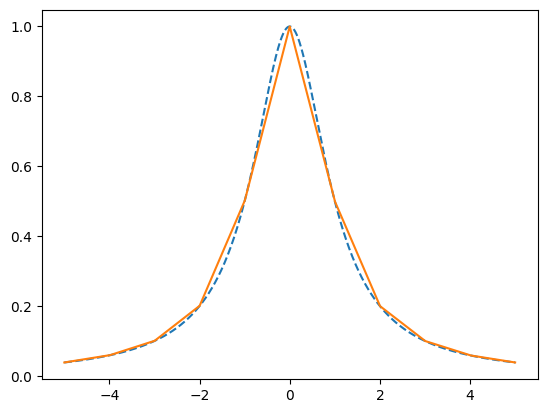
\includegraphics[width=5cm]{c1.png}
    \caption{线性}
    \label{c1}
\end{minipage}
\qquad
\begin{minipage}{5cm}
    \centering
    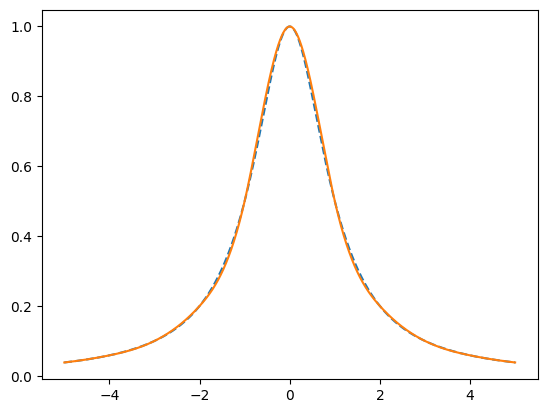
\includegraphics[width=5cm]{c3.png}
    \caption{自然}
    \label{c2}
\end{minipage}
\begin{minipage}{5cm}
    \centering
    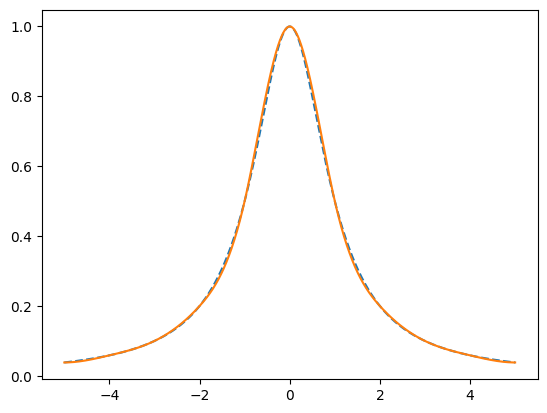
\includegraphics[width=5cm]{c2.png}
    \caption{完全}
    \label{c3}
\end{minipage}
\qquad
\begin{minipage}{5cm}
    \centering
    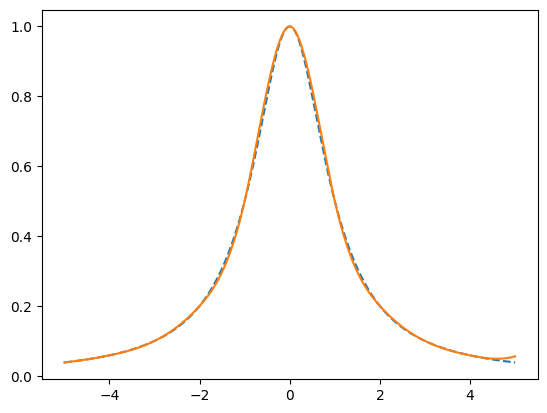
\includegraphics[width=5cm]{c4.png}
    \caption{端点处二阶导指定}
    \label{c4}
\end{minipage}
\begin{minipage}{5cm}
    \centering
    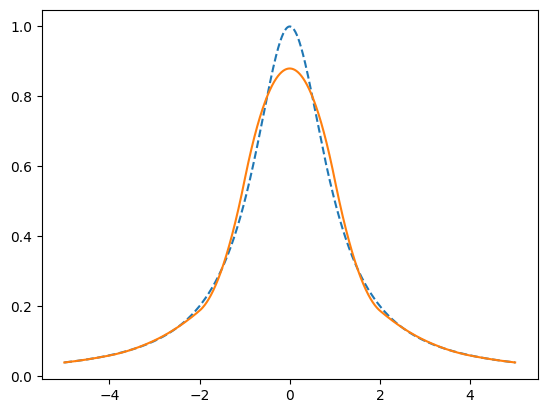
\includegraphics[width=5cm]{c5.png}
    \caption{二次}
    \label{c5}
\end{minipage}
\end{figure}

D 题的答案存入了 \verb|d.csv| 中。如下表。

$E_L,E_C,E_N,E_S,E_Q$ 分别为分段线性样条、自然样条、完全样条、端点处二阶导指定的样条、分段二次样条的误差。

\begin{tabular}{|c|c|c|c|c|c|} \hline
$x$ & $E_L$ & $E_C$ & $E_N$ & $E_S$ & $E_Q$  \\ \hline
-3.5 & 0.00394007 & 4.14009e-05 & 0.000669568 & 0.00068675 & 2.87991e-18 \\ \hline
-3 & 5.54976e-18 & 5.54976e-18 & 5.54976e-18 & 5.54976e-18 & 0.00141838 \\ \hline
-0.5 & 0.05 & 0.02052 & 0.0205289 & 0.0205291 & 4.43981e-17 \\ \hline
0 & 0 & 0 & 1.11022e-16 & 0 & 0.120238 \\ \hline
0.5 & 0.05 & 0.02052 & 0.0205289 & 0.0205291 & 6.66242e-17 \\ \hline
3 & 5.54976e-18 & 1.94275e-17 & 5.54976e-18 & 1.94275e-17 & 0.00141838 \\ \hline
3.5 & 0.00394007 & 4.14009e-05 & 0.000669568 & 0.00068675 & 1.67577e-17 \\ \hline
\end{tabular}

在线性样条和三次样条的结点(-3,0,3)处,$E_L,E_C,E_N,E_S$ 的值都为零或接近系统误差;在二次样条的结点(-3.5,-0.5,0.5,3,5)处,$E_Q$ 的值接近系统误差。而在线性样条和三次样条两个结点的中点处,线性样条和三次样条都有较大的误差,特别是在 $\pm 0.5$ 处分别达到了 $0.05$ 和 $0.02$。在二次样条两个结点的中点处,二次函数则有较大误差,特别是在 $0$ 处达到了 $0.12$。

\section{曲线拟合(E题)}

对于曲线拟合的问题,一般的处理方法是建立曲线的参数方程 $x(t),y(t)$,然后对这两个函数分别进行拟合得到两个样条函数 $\hat{x}(t),\hat{y}(t)$。由于参数方程的建立方法多种多样,且实际应用时曲线会存在奇点(例如本题),因此很难对一般曲线拟合问题设计出通用的方法,只能具体问题具体分析。

\subsection{心形曲线拟合}

心形线曲线的方程为

\begin{equation}
    x^2+(\dfrac 32y-\sqrt{|x|})^2=3.
\end{equation}

由极坐标可得

\begin{equation}
    x(t)=\sqrt{3} sin t,y(t)=\dfrac 23(\sqrt 3\cos t+\sqrt{\sqrt 3|\sin t|})
\end{equation}

这样就建立了心形曲线的参数方程。

按题目要求使用累计弧长参数,故将曲线重新参数化。

\begin{equation}
    s(t)=\int_0^t\sqrt{x'(\tau)^2+y'(\tau)^2}d\tau
\end{equation}

但这个积分是没有原函数的,更不能显示解出 $t$。但注意到我们并不需要求出 $t$ 关于 $s$ 的表达式,只需求出 $s$ 取值为 $\dfrac kn L,k=1,2,\dots,n-1$ 的值进而求出结点处的 $t$ 值(其中 $L$ 为总弧长),然后以这些 $t$ 为结点构造样条函数。

所以问题转化为求解 $n-1$ 个方程 $s(t)=\dfrac kn L$。它等价于

\begin{equation}
    \int_{t_k}^{t_{k+1}}\sqrt{x'(\tau)^2+y'(\tau)^2}d\tau=\dfrac kn L
\end{equation}

这是一个非线性方程。因为 $s$ 的导数难以求出,故可以使用第一章的二分法或割线法求解(本文使用二分法)。

最后一个问题就是 $s(t)$ 是一个不能直接计算的积分,因此我们利用第六章的辛普森积分计算。但被积分式在积分边界处是奇异的,直接用二次函数拟合效果很差,即使用复化辛普森公式分段收敛速度也非常慢。因此采用自适应辛普森积分,即当 $|I^S_{l,r}(s)-(I^S_{l,\frac {l+r}2}(s)+I^S_{\frac {l+r}2,r}(s)|<\varepsilon$ 时直接取 $I^S_{l,r}(s)$ 作为 $(l,r)$ 上积分的近似,否则取中点,两边分别继续分治计算。

分别用分段线性样条和自然样条进行拟合(代码见 E.cpp):

\begin{lstlisting}[language={c++}]
#include <bits/stdc++.h>
#include "Spline.h"
#include "../HW1/function.h"
using namespace std;

const double PI = acos(-1), Q = sqrt(3), dt = 1e-8, eps = 1e-12;

class X : public Function<double> {
public:
	virtual double operator () (const double& t) const {
		return Q * sin(t);
	}
	virtual double d(const double& t) const {
		return Q * cos(t);
	}
} x;

class Y : public Function<double>{
public:
	virtual double operator () (const double& t) const {
		return 2 * (Q * cos(t) + sqrt(Q * fabs(sin(t)))) / 3;
	}
	virtual double d(const double& t) const {
		if (sin(t) > 0) return 2 * (-Q * sin(t) + sqrt(Q) * cos(t) / 2 / sqrt(fabs(sin(t)))) / 3;
		else return 2 * (-Q * sin(t) - sqrt(Q) * cos(t) / sqrt(fabs(sin(t)))) / 3;
	}
} y;

class S : public Function<double>{
public:
	virtual double operator () (const double& t) const {
		return sqrt(x.d(t) * x.d(t) + y.d(t) * y.d(t));
	}
} s;

// (l, r) 上的辛普森积分
double IS(const Function<double>& f, const double& l, const double& r) {
	return (r-l) * (f(l) + 4 * f((l+r)/2) + f(r)) / 6;
}
// 自适应辛普森积分
double Simpson(const Function<double>& f, const double& l, const double& r) {
	double mid = (l+r) / 2, s = IS(f, l, r), t = IS(f, l, mid) + IS(f, mid, r);
	if (fabs(s-t) < eps) return s;
	return Simpson(f, l, mid) + Simpson(f, mid, r);
}

// 求出曲线的 n 等分点
vector<double> Get_Knots(int n) {
	double I = Simpson(s, dt, PI - dt) * 2;
	vector<double> x(n+1), y(n+1);
	x[0] = dt;
	// 在曲线上按长度均匀取插值结点
	for (int i = 1; i <= n/2-1; ++ i) {
		double l = x[i-1], r = 2*PI;
		while(r-l>=1e-8){
			double mid = (l+r) / 2;
			double Im = Simpson(s, x[i-1], mid);
			if (Im < I/n) l = mid;
			else r = mid;
		}
		x[i] = l;
	}
	x[n/2] = PI - dt;
	for (int i = 0; i <= n/2-1; ++ i) {
		x[n-i] = 2*PI - x[i];
	}
	return x;
}

// 用线性样条拟合曲线
// file 曲线数据的文件名
void Linear_heart_plot(int n, int m, const char* file) {
	vector<double> t = Get_Knots(n), f(n+1), g(n+1);
	for (int i = 0; i <= n; ++ i) f[i] = x(t[i]);
	for (int i = 0; i <= n; ++ i) g[i] = y(t[i]);
	LinearSpline<double> X = LinearSpline<double>(t, f);
	LinearSpline<double> Y = LinearSpline<double>(t, g);
	ofstream out(file);
	out << "x,y" << '\n';
	for (int i = 0; i <= m; ++ i) out << X.GetValue(dt+(2*PI-2*dt)*i/m) << ',' << Y.GetValue(dt+(2*PI-2*dt)*i/m) << '\n';
}

// 用三次样条拟合曲线(这里只实现了自然三次样条)
void Cubic_heart_plot(int n, int m, const string& mode, const char* file) {
	vector<double> t = Get_Knots(n), f(n+1), g(n+1);
	for (int i = 0; i <= n; ++ i) f[i] = x(t[i]);
	for (int i = 0; i <= n; ++ i) g[i] = y(t[i]);
	double m0 = 0, mn = 0;
	CubicSpline<double> X = CubicSpline<double>(t, f, mode, m0, mn);
	CubicSpline<double> Y = CubicSpline<double>(t, g, mode, m0, mn);
	ofstream out(file);
	out << "x,y" << '\n';
	for (int i = 0; i <= m; ++ i) out << X.GetValue(dt+(2*PI-2*dt)*i/m) << ',' << Y.GetValue(dt+(2*PI-2*dt)*i/m) << '\n';
}

int main() {
	Linear_heart_plot(10, 50000, "e1.csv");
	Linear_heart_plot(40, 50000, "e2.csv");
	Linear_heart_plot(160, 50000, "e3.csv");
	Cubic_heart_plot(10, 50000, "Natural", "e4.csv");
	Cubic_heart_plot(40, 50000, "Natural", "e5.csv");
	Cubic_heart_plot(160, 50000, "Natural", "e6.csv");
}
\end{lstlisting}

拟合效果如下。线性和自然样条见图 \ref{e1} 和图 \ref{e2}。蓝色、黄色、绿色的曲线分别是拟合点数为 $n=10,40,160$ 的曲线:

\begin{figure}[htbp]
\centering
\begin{minipage}{5cm}
    \centering
    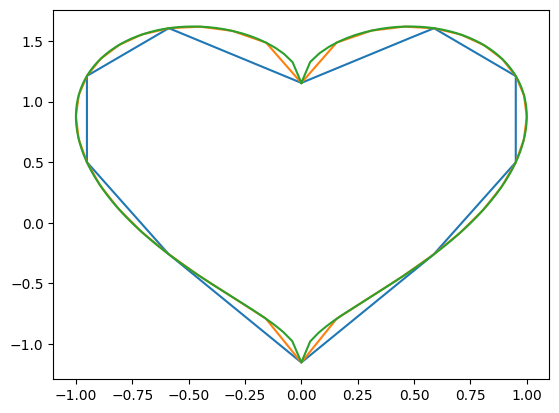
\includegraphics[width=5cm]{e1.png}
    \caption{线性}
    \label{e1}
\end{minipage}
\qquad
\begin{minipage}{5cm}
    \centering
    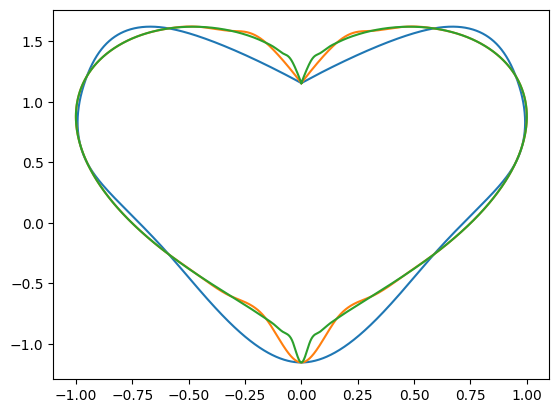
\includegraphics[width=5cm]{e2.png}
    \caption{自然}
    \label{e2}
\end{minipage}
\end{figure}

$n=10$ 和 $n=40$ 时,两种样条的表现都很差;$n=160$ 时,样条在远离 $x=0$ 的区域拟合效果很好,但在 $x=0$ 附近拟合效果很差。这是因为在 $x=0$ 附近 $y$ 的导数趋向于无穷大,拟合问题本身的条件数很大,不能期望算法的拟合效果很好。

需要注意的是,对于心形曲线,不能直接用完全样条或端点处二阶导指定的样条拟合,因为它们需要取到 $t=0$ 处的导数值,而此时 $|y'(t)|\rightarrow \infty$。当然,注意到本题拟合的曲线是周期的,因此可任选其他的端点(例如 $\dfrac \pi 2$),这样得到的结果和自然样条是类似的。但这样就失去了完全样条的优势(固定端点的斜率),所以这里不做实现。

\end{document}